\chapter{Track Laydown}
\label{chap:track-laydown}

One of the often overlooked aspects of \ac{MOC} implementations is the method chosen to lay down tracks across the geometry. In Chapter~\ref{chap:moc} the basic strategy of laying down tracks and then applying the \ac{MOC} equations over the tracks was discussed. In this chapter, the strategies for laying down tracks are discussed in great detail. First, this chapter discusses 2D track laydown in Section~\ref{sec:laydown-2D} which is relatively straightforward. Section~\ref{sec:angular-quadrature} discusses how angular quadratures are formed and the impact of track linking requirements. Then, Section~\ref{sec:laydown-3D} describes how a 2D track laydown can be used to form a 3D track laydown. Section~\ref{sec:openmoc-laydown} details features of the OpenMOC track generation implementation. This chapter closely follows the track laydown analysis of Shaner, et al~\cite{shaner-laydown}.

\section{2D Track Generation}
\label{sec:laydown-2D}

As presented in Chapter~\ref{chap:moc}, \ac{MOC} lays tracks across the geometry over which the \ac{MOC} equations are applied. While one dimensional, each track represents a particular three dimensional volume and angular subspace. The first step in setting up the \ac{MOC} problem is creating tracks that span the spatial and angular space of the problem.

When creating the tracks, it is important to consider the boundary conditions as these determine whether the outgoing angular flux needs to be passed as the incoming flux to another track. For flexibility, OpenMOC focuses on generating tracks that are cyclic and can therefore be used for reflective, periodic, or vacuum boundary conditions. While analysis of full-core problems typically involves only vacuum boundaries, it is helpful to have the option for reflective boundaries to compare the results of small-core benchmarks, such as the C5G7 benchmark~\cite{c5g7}, to other codes. 

In this discussion, it is important to make clear the distinction between tracks and segments (sometimes also referred to as intersections). Tracks are defined to span an entire geometry or geometry sub-domain and pass through region boundaries. On the other hand, segments do not cross region or material boundaries.

Tracks for a 2D \ac{MOC} problem are typically laid down using the cyclic tracking approach. Users input a desired radial ray spacing $\tilde{\delta}_\phi$ and number of azimuthal angles $n_{\phi}$ in $[0, 2 \pi]$. With this approach, desired azimuthal angles are created to evenly subdivide the angular space such that the $i^{\text{th}}$ desired azimuthal angle $\tilde{\phi}_i$ in $[0, \frac{\pi}{2}]$ is paired with a complementary azimuthal angle $\tilde{\phi}_{\frac{n_{\phi}}{2} - i - 1}$ as described in Eq.~\ref{eq:disc-azim-angles} and Eq.~\ref{eq:disc-azim-angles-comp}.
\begin{equation}
\tilde{\phi}_i = \frac{2 \pi}{n_\phi} \left(\frac{1}{2} + i\right) \qquad \forall \qquad i = \Big[0,\frac{n_{\phi}}{2}\Big)
\label{eq:disc-azim-angles}
\end{equation}
\begin{equation}
\tilde{\phi}_{\frac{n_{\phi}}{2} - i - 1} = \pi - \tilde{\phi}_i \qquad \forall \qquad i= \Big[0,\frac{n_{\phi}}{4}\Big)
\label{eq:disc-azim-angles-comp}
\end{equation} 
Other valid angular quadrature sets can also be used~\cite{3D-MOC-annals}. By tracking both forward and backward along a track, the full $2 \pi$ angular space is covered as shown in Fig. \ref{fig:laydown-2D} for four azimuthal angles. Tracks are laid down such that they intersect with a complementary track at the boundaries. 

\begin{figure}[h!]
	\centering
	\begin{subfigure}{0.35\textwidth}
		\centering
		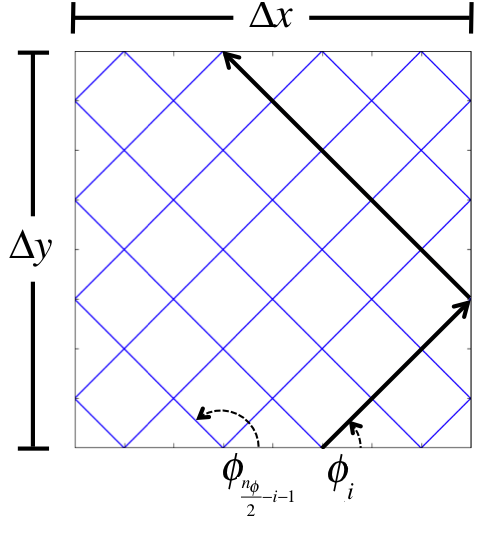
\includegraphics[width=\linewidth]{figures/laydown/fwd_bwd_tracking_a.png}
		\caption{}
		\label{fig:laydown-2D-a}
	\end{subfigure}
	\begin{subfigure}{0.35\textwidth}
		\centering
		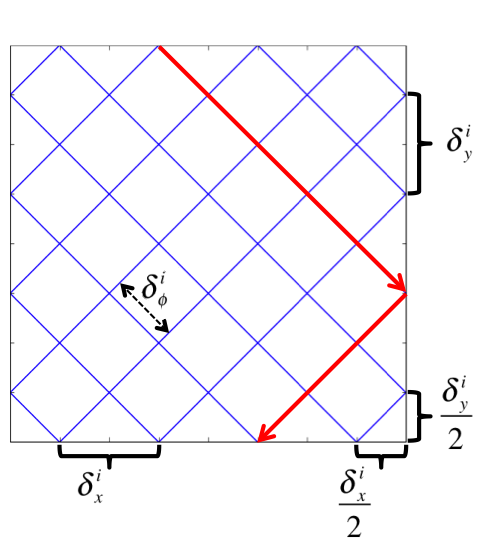
\includegraphics[width=\linewidth]{figures/laydown/fwd_bwd_tracking_b.png}
		\caption{}
		\label{fig:laydown-2D-b}
	\end{subfigure}
	\caption[]{Illustration of (a) forward and (b) backward tracking for 2D \ac{MOC} track laydown. The geometry has dimensions $\Delta x \times \Delta y$.}
	\label{fig:laydown-2D}
\end{figure}

In order to guarantee cyclic wrapping of 2D tracks, there must be an integer number of tracks on $x$ and $y$ axes for each azimuthal angle. This requires the actual spacing between tracks be chosen as:
\begin{equation}
\delta_x^i = \frac{\Delta x}{n_x^i} \qquad \delta_y^i = \frac{\Delta y}{n_y^i}
\label{eq:3DGT-dx-dy}
\end{equation}
where $n_x^i$ is the integer number of tracks along the $x$-axis for the $i^{\textit{th}}$ azimuthal angle. The same notation applies to the $y$ direction. Using the input value of $\tilde{\delta}_{\phi}$, the integer number of tracks along the axes for the $i^{\textit{th}}$ azimuthal angle are computed as:
\begin{equation}
n_x^i = \Bigg\lceil\Bigg(\frac{\Delta x \sin{\tilde{\phi}_i}}{\tilde{\delta}_\phi}\Bigg)\Bigg\rceil \qquad n_y^i = \Bigg\lceil\Bigg(\frac{\Delta y \cos{\tilde{\phi}_i}}{\tilde{\delta}_\phi}\Bigg) \Bigg\rceil
\label{eq:3DGT-nx-ny}
\end{equation}
where the ceiling is taken to ensure at least one track intersects with each axis. The azimuthal angle also needs to be corrected as:
\begin{equation}
\phi_i = \tan^{-1} \bigg(\frac{\delta_y^i}{\delta_x^i}\bigg)
\label{eq:azi-correct}
\end{equation}
where $\phi_i$ is used to denote the $i^{\textit{th}}$ corrected azimuthal angle. Using the corrected azimuthal angle, the radial ray spacing for each angle is also corrected as:
\begin{equation}
\delta_{\phi}^i = \delta_x^i \sin{\phi_i}
\label{eq:azi-space-correct}
\end{equation}
where $\delta_{\phi}^i$ is used to denote the corrected radial ray spacing. Using the corrected values, $\phi_i$ and $\delta_{\phi}^i$, the 2D tracks are laid down on the geometry. 


\section{Angular Quadrature}
\label{sec:angular-quadrature}

In any \ac{MOC} implementation, angular quadratures needed. A angular quadrature is a set of angles and weights that can accurately integrate the angular space. In this thesis, a product quadrature is assumed which allows azimuthal and polar quadratures to be separable. For a given azimuthal and polar angle combination, the weight from the azimuthal quadrature is multiplied with the weight from the polar quadrature to determine the total angular weight.

\subsection{Azimuthal Quadrature}

For the azimuthal space, equal angle separation is chosen since it is expected that all azimuthal directions are equally important, as given in Eq.~\ref{eq:disc-azim-angles}. The angles needed to be corrected to ensure track linking at reflective and periodic boundaries. Azimuthal weights $w_{\phi}^i$ for azimuthal index $i=1...{n_\phi/2}$ are then chosen as
\begin{equation}
w_{\phi}^i = \frac{\phi_{i+1} - \phi_{i-1}}{4\pi}
\end{equation}
with the virtual angles $\phi_{0}$ and $\phi_{n_\phi/2+1}$ are defined to be
\begin{equation}
\phi_0 = - \phi_1 \qquad \phi_{n_\phi/2+1} = \pi - \phi_{n_\phi/2}
\end{equation}
In this form, the weights account for the angular space represented by each track. Note that these relationships define weights for azimuthal angles $\phi \in [0, \pi]$ since tracking both forward and backward along tracks accounts for the full $2\pi$ azimuthal space.

\subsection{Polar Quadrature}

In 2D, the axial dimension is assumed infinite and therefore linking is not required beyond the radial plane. This allows any polar angle quadrature to be chosen without having to correct polar angles. One interpretation is that tracks in 2D \ac{MOC} are allowed to continue unbounded axially, with their $z$-height insubstantial, since behavior must be the same along the axial direction due to symmetry. Popular quadratures include the Gauss-Legendre polar quadrature and the TY quadrature~\cite{ty-quadrature}. Both are important polar quadrature sets for \ac{MOC} solvers.

The Gauss-Legendre quadrature set is based on the Gaussian quadrature rule which allows polynomials of order up to $2n-1$ to be integrated exactly using only $n$ quadrature points. The Gauss-Legendre quadrature set chooses quadrature points and weights to enforce the exact integration of Legendre polynomials of order $2n-1$ over the interval [-1, 1] with $n$ points. This is accomplished by choosing quadrature points $x_j$ and weights $w_{\textit{gl}}^j$ such that
\begin{equation}
\int_{-1}^{1} dx \, P_m(x) = \sum_{j=1}^n x_j w_{\textit{gl}}^j \qquad \forall m = [0, 2n-1]
\end{equation}
where $P_m(x)$ is the Legendre polynomial of order $m$. The quadrature points $x_j$ are chosen to be the roots of the Legendre polynomial $P_n(x)$ and the weights $w_{\textit{gl}}^j$ are computed as
\begin{equation}
w_{\textit{gl}}^j = \frac{2(1-x_j^2)}{(n+1)^2\left[P_{n+1}(x_j)\right]^2}
\end{equation}
Since the polar angle $\theta \in [0, \pi]$ and $\cos{\theta} \in [-1, 1]$, this quadrature rule can be used by the taking polar angles to be $\cos^{-1} x_j$.  

Another useful quadrature for 2D \ac{MOC}, and the most widely used in production \ac{MOC} codes, is the TY polar quadrature~\cite{ty-quadrature}. This quadrature set notes the relation of \ac{MOC} to collision probability methods, allowing an analytic form for \ac{MOC} scalar fluxes in terms of collision probabilities. These collision probabilities can then be cast in terms of \ac{MOC} equations along a strip associated with a 2D track to show that the polar quadrature is optimal when it minimizes the error of approximating Bickley functions. With this insight, the TY quadrature is computationally formed by minimizing the error to Bickley functions, which can be numerically evaluated. In practice, most codes take the results of the published optimization to hard-code the polar angle quadrature points and associated polar weights. While the TY quadrature has been quite successful in 2D simulations, it cannot be easily extended to 3D \ac{MOC} since it relies on an analytic form for the neutron transport over a 2D strip. Therefore, the Gauss-Legendre quadrature is typically used in 3D \ac{MOC} simulations. 

Together, the azimuthal and polar quadrature combine to form a product quadrature. An example of a quadrature for 3D MOC is shown in Figure~\ref{fig:quad-unit-sphere} where the product quadrature is plotted on a octant of the unit sphere using the Gauss-Legendre polar quadrature.

\begin{figure}[h!]
	\centering
	\begin{subfigure}{0.3\textwidth}
		\centering
		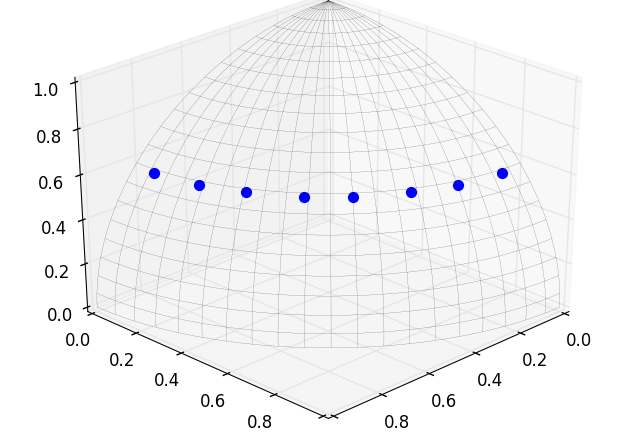
\includegraphics[width=\linewidth]{figures/laydown/GL_2.png}
		\caption{}
		\label{fig:quad-unit-sphere-a}
	\end{subfigure}
	\begin{subfigure}{0.3\textwidth}
		\centering
		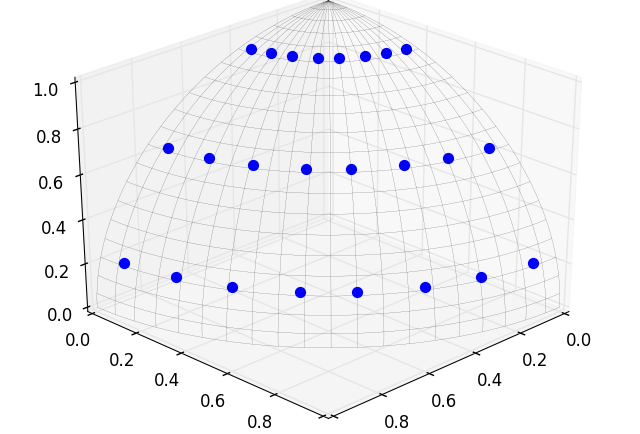
\includegraphics[width=\linewidth]{figures/laydown/GL_6.png}
		\caption{}
		\label{fig:quad-unit-sphere-b}
	\end{subfigure}
	\begin{subfigure}{0.3\textwidth}
		\centering
		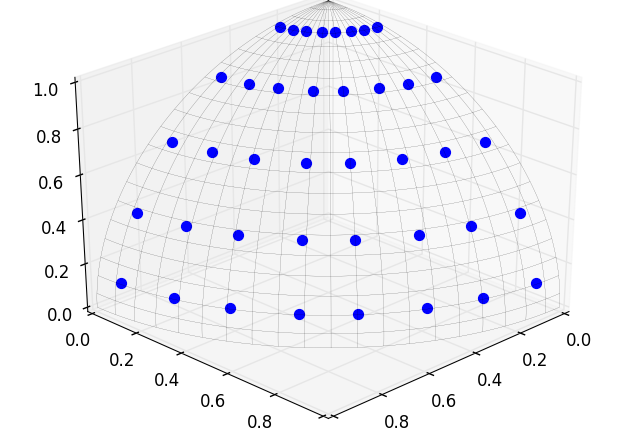
\includegraphics[width=\linewidth]{figures/laydown/GL_10.png}
		\caption{}
		\label{fig:quad-unit-sphere-c}
	\end{subfigure}
	\caption[]{Illustration of a product quadrature for a 3D MOC problem on an octant of the unit sphere with the Gauss Legendre polar quadrature using 32 azimuthal angles and (a) 2 polar angles, (b) 6 polar angles, and (c) 10 polar angles.}
	\label{fig:quad-unit-sphere}
\end{figure}


\section{3D Track Generation}
\label{sec:laydown-3D}

Once the 2D tracks are laid down, 3D tracks can be formed from the 2D tracks. In generating 3D tracks, it is assumed that 3D tracks are laid down as $z$-stacked arrays of tracks that project down onto the 2D track layout. A sparse 2D and associated 3D track laydown for a homogeneous cube geometry is illustrated in Fig~\ref{fig:sample-tracks}.

\begin{figure}[h!]
	\centering
	\begin{subfigure}{0.25\textwidth}
		\centering
		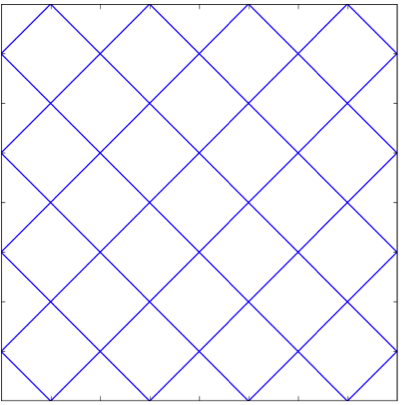
\includegraphics[width=\linewidth]{figures/laydown/sample-tracks_a.png}
		\caption{}
		\label{fig:sample-tracks-a}
	\end{subfigure}
	\begin{subfigure}{0.35\textwidth}
		\centering
		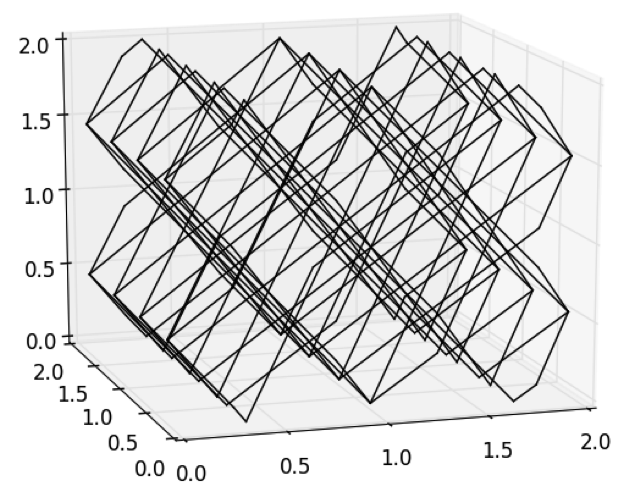
\includegraphics[width=\linewidth]{figures/laydown/sample-tracks_b.png}
		\caption{}
		\label{fig:sample-tracks-b}
	\end{subfigure}
	\caption[]{Illustration of (a) 2D and (b) 3D  tracks for a homogeneous cube geometry.}
	\label{fig:sample-tracks}
\end{figure}


\subsection{Requirements for Cyclic Track Laydown in 3D}

Before discussing the conditions required to generate cyclic tracks in 3D, it is important to understand the concept of a track cycle. Fig.~\ref{fig:tracks-cycles-2D} shows a track laydown in 2D for reflective track cycles with $T_{R,k}^{i}$ denoting the $k^{\textit{th}}$ reflective track cycle for the $i^{\textit{th}}$ azimuthal angle. 

% insert picture
\begin{figure}[h]
	\centering
	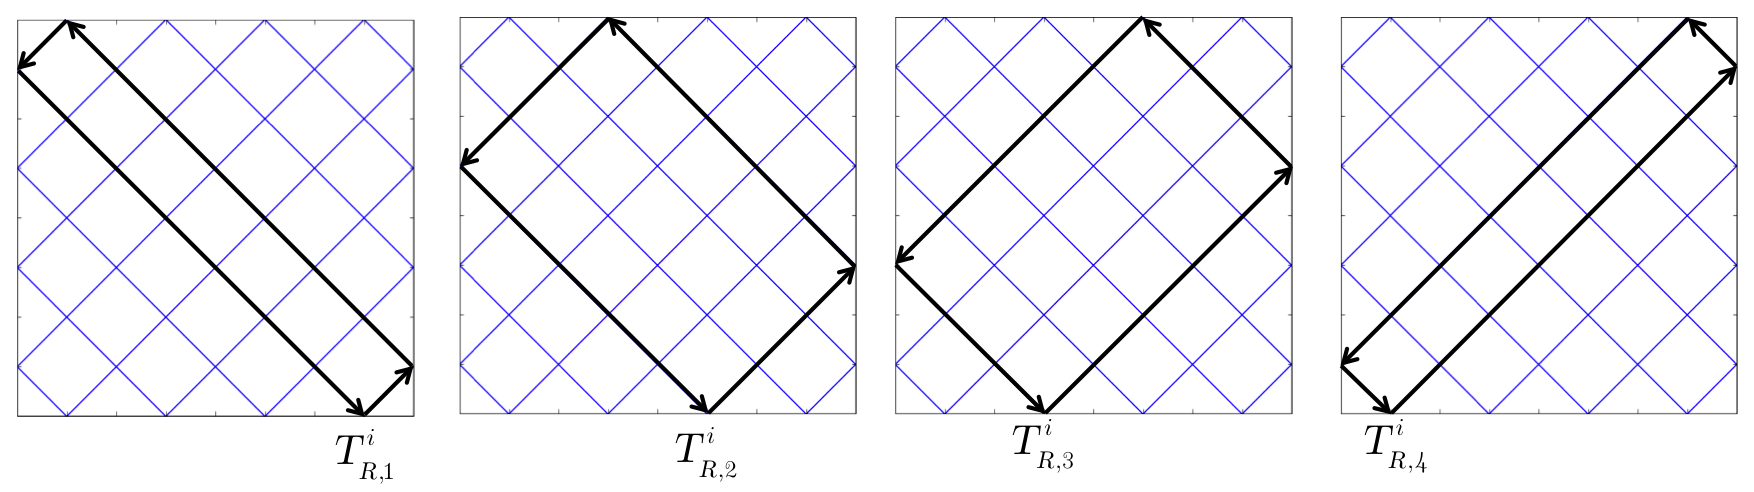
\includegraphics[width=6.5in]{figures/laydown/reflective-track-cycles-3.png}
	\caption{An illustration of track cycles. Each plot highlights one of the 2D track cycles labeled $T_{R,k}^{i}$ denoting the $k^{th}$ track cycle for the $i^{\textit{th}}$ azimuthal angle.}
	\label{fig:tracks-cycles-2D}
\end{figure}


To generate 3D tracks, users input a desired track axial ray spacing $\tilde{\delta}_z$ and number of polar angles $n_{\theta}$ in $[0, \pi]$ in addition to the parameters required to generate 2D tracks. With this approach, desired polar angles are created according to the chosen polar quadrature set. In OpenMOC, it is assumed that quadrature sets are symmetric such that the desired polar angle $\tilde{\theta}_{j}$ with polar angle index $j$ follows
\begin{equation}
\tilde{\theta}_{j} = \pi - \tilde{\theta}_{n_{\theta} - j - 1} \qquad \forall \qquad j= \Big[0,\frac{n_{\theta}}{2}\Big),
\end{equation} 
where $\tilde{\theta}_{n_{\theta} - j - 1}$ is the complement of the desired polar angle. Most useful quadrature sets, such as the Gauss Legendre quadrature set, are indeed symmetric. 

Note that the polar angles are initially defined to be independent of azimuthal angle index. Later, the corrected polar angle will be dependent on the azimuthal angle to ensure the tracks are cyclic. Following the same notation used to describe the azimuthal angles, the corrected polar angles will be denoted by $\theta_{i,j}$ for azimuthal index $i$ and polar index $j$. By tracking both forward and backward along a track, the full $4 \pi$ angular space can be covered as previously shown in Fig.~\ref{fig:sample-tracks} for four azimuthal and two polar angles.

Tracks are laid down such that they intersect with a complementary track at the boundaries. Selecting an arbitrary cycle $T_{R,k}^{i}$ a set of 3D tracks are followed as they complete one 2D cycle. Fig.~\ref{fig:projected-tracks} highlights a particular 2D track cycle and a set of 3D tracks projected along that cycle.

\begin{figure}[h!]
	\centering
	\begin{subfigure}{0.35\textwidth}
		\centering
		\vspace{0.15in}
		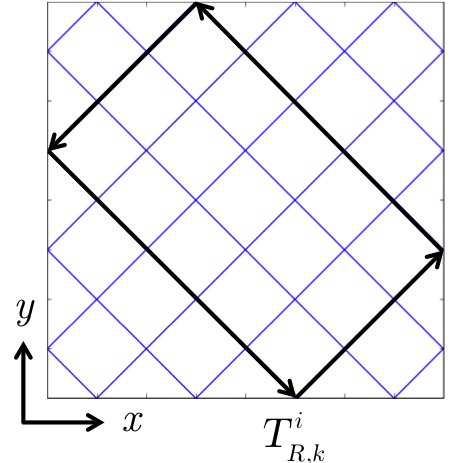
\includegraphics[width=\linewidth]{figures/laydown/track_cycles_3_a.png}
		\caption{}
		\label{fig:projected-tracks-a}
	\end{subfigure}
	\begin{subfigure}{0.45\textwidth}
		\centering
		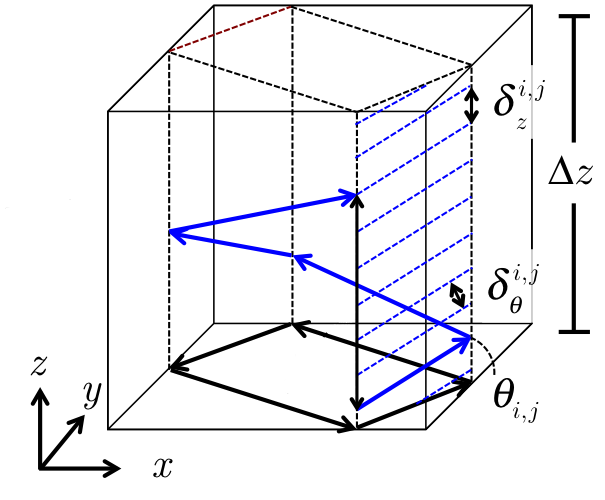
\includegraphics[width=\linewidth]{figures/laydown/track_cycles_3_b.png}
		\caption{}
		\label{fig:projected-tracks-b}
	\end{subfigure}
	\caption[]{Illustration of (a) an arbitrary 2D track cycle $T_{R,k}^{i}$ and (b) a set of 3D tracks projected along the 2D track cycle.}
	\label{fig:projected-tracks}
\end{figure}


To guarantee cyclic track wrapping of the 3D tracks, two conditions must be met:

\begin{enumerate}
	\item The distance between the beginning and end of a 3D track projection along a 2D track cycle must be an integer number of track spacings for each 3D cycle.
	\item There must be an integer number of track spacings along the $z$-axis over the depth of geometry, $\Delta z$ for each azimuthal/polar angle combination.
\end{enumerate}

The first condition guarantees that a 3D track cycle wraps back onto another 3D track when the 2D reflective cycle is completed. The second condition guarantees that a 3D track cycle that contains a reflection off a top or bottom surface still reflects into an existing 3D track when the 2D cycle is completed. All 3D track generation schemes must comply with these conditions, though many make additional assumptions.

\subsection{The Modular Ray Tracing Method}

\ac{MRT} uses the previously stated conditions for 3D cyclic ray tracing to generate tracks for a rectangular geometry. After the 2D track information has been generated, the 3D track information can be computed using the requirements for 3D cyclic tracking. \ac{MRT} relies on the principle that a geometry can be uniformly decomposed into a series of rectangular cuboids of equal dimensions. For a domain, the number of tracks and spacing between tracks in $x$ and $y$ are described in Eq.~\ref{eq:mrt-nx-ny} and Eq.~\ref{eq:mrt-dx-dy}, respectively,

\begin{equation}
n_x^i = \Bigg\lceil\frac{\Delta x\sin{\tilde{\phi}_i}}{D_x \tilde{\delta}_\phi}\Bigg\rceil \qquad n_y^i = \Bigg\lceil\frac{\Delta y \cos{\tilde{\phi}_i}}{D_y \tilde{\delta}_\phi} \Bigg\rceil
\label{eq:mrt-nx-ny}
\end{equation}

\begin{equation}
\delta_x^i = \frac{\Delta x}{D_x n_x^i} \qquad \delta_y^i = \frac{\Delta y}{D_y n_y^i},
\label{eq:mrt-dx-dy}
\end{equation}

\noindent
where $D_x$ and $D_y$ are the integer number of domains in the $x$ and $y$ directions, respectively. This guarantees that an integer number of tracks lie along the $x$ and $y$ boundaries of each domain cell and that tracks on one surface line up with adjoining tracks in the neighbor domain cell. 

When generating tracks using the \ac{MRT} method, it is important to remember that a track crossing a domain interface needs to connect with another track on the neighboring domain. Following a series of tracks across the geometry, notice that the series of tracks is periodic. A periodic track cycle is defined to be the series of domain tracks that repeats when a global track traverses a geometry. Fig.~\ref{fig:periodic-cycles} shows the periodic track cycles for one azimuthal angle in our sample geometry when it is split into four domains.

% insert picture
\begin{figure}[h]
	\centering
	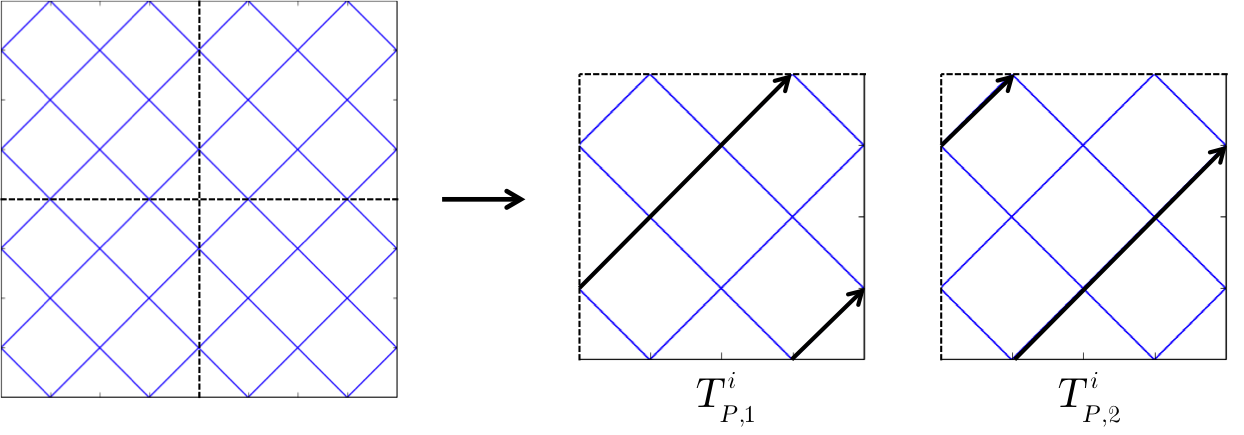
\includegraphics[width=5in]{figures/laydown/2d_periodic_track_cycles_2.png}
	\caption{An illustration of 2D periodic track cycles $T_{P,k}^i$ for the $k^{th}$ periodic track cycle with the azimuthal index $i$ in a sample geometry split into four domains.}
	\label{fig:periodic-cycles}
\end{figure}
Note that all 2D track cycles for a particular azimuthal angle index $i$ have the same periodic cycle length $L_P^{i}$ that can be computed as
\begin{equation}
L_P^i = \frac{\delta_x^i}{\cos{\phi_i}}  \text{lcm} \bigg( n_x^i, \,  \frac{\Delta y}{D_y \delta_x^i \tan{\phi_i}} \bigg),
\label{eq:period-cycle-len}
\end{equation}

\noindent
where lcm is the least common multiple. Using the periodic cycle length for each azimuthal angle, the integer number of track spacings $n_l^{i,j}$ between the beginning and end of a set of 3D tracks after one complete 2D cycle can be computed as
\begin{equation}
n_l^{i,j} = \Bigg\lceil \frac{L_P^i \cot{\tilde{\theta}_{j}}}{\tilde{\delta}_z} \Bigg\rceil,
\label{eq:MRT-nl}
\end{equation}

\noindent
where the subscript $l$ is used to signify that $n_l^{i,j}$ is measured along the direction of a track cycle. Next, the number of track spacings along the $z$-axis needs to be set to an integer number. The number of tracks on the $z$-axis can be found by considering the relation between the number of track spacings in the $z$-direction and the spacing along the length of the 2D track in Eq.~\ref{eq:tan-theta}.

\begin{equation}
\tan{\tilde{\theta}_{j}} = \frac{\delta_L^i}{\tilde{\delta}_z} = \frac{L_P^i}{n_l^{i,j}} \frac{n_z^{i,j}}{\Delta z}
\label{eq:tan-theta}
\end{equation}

\noindent
Rearranging and inserting the desired polar angle $\tilde{\theta}_{i,j}$, this equation yields an expression for the number of tracks $n_z^{i,j}$ on the $z$-axis as

\begin{equation}
n_z^{i,j} = \Bigg\lceil\frac{\Delta z n_l^{i,j} \tan{\tilde{\theta}_{i,j}}}{L_P^i} \Bigg\rceil,
\label{eq:MRT-nz}
\end{equation}

\noindent
where the ceiling ensures at least one track crossing on the $z$-axis. The corrected $z$-spacing $\delta_z^{i,j}$ between 3D tracks is computed in Eq.~\ref{eq:MRT-delta-z}.

\begin{equation}
\delta_z^{i,j} = \frac{\Delta z}{n_z^{i,j}}
\label{eq:MRT-delta-z}
\end{equation}

\noindent
Using the 2D cycle length and number of track crossings on the $z$-axis and along the length of the 2D cycle, the polar angle can be corrected using Eq.~\ref{eq:MRT-theta-correct}.

\begin{equation}
\theta_{i,j} = \tan^{-1} \bigg( \frac{L_P^i}{n_l^{i,j} \delta_z^{i,j}}\bigg)
\label{eq:MRT-theta-correct}
\end{equation}
It is important to note that when polar angles are adjusted, the Gauss-Legendre quadrature set no longer is guaranteed to exactly integrate Legendre polynomials of order up to $2n-1$ with $n$ quadrature points. In fact, it is not guaranteed to exactly integrate any Legendre polynomials beyond the zeroth order. This could either be ignored, assuming that the quadrature can still integrate Legendre polynomials of order up to $2n-1$ with reasonable accuracy, or the weights can be re-computed to ensure that Legendre polynomials of order $n$ are exactly integrated. Both options are implemented in OpenMOC. The angular track weight $\alpha_t$ of track $t$ with azimuthal angle index $i$ and polar index $j$ using a Gauss Legendre quadrature can be computed as
\begin{equation}
\alpha_t = w_{\phi}^i w_{\textit{gl}}^j .
\end{equation}

The procedure for identifying the periodic track cycles and finding the start and end points for all tracks using the \ac{MRT} method can seem a bit tedious, so others have simplified the \ac{MRT} method by noticing that the lengths of all 2D tracks are an integer multiple of the shortest 2D track \cite{kochunas}. For example, the length of the first three 2D tracks, $t_1^i$, $t_2^i$, and $t_3^i$, for azimuthal index $i$ are shown in Eq.~\ref{eq:short-track}, Eq.~\ref{eq:short-track-2}, and Eq.~\ref{eq:short-track-3}.

\begin{equation}
l_1^i = \sqrt{\bigg[\frac{\delta_x^i}{2}\bigg]^2 + \bigg[\frac{\delta_y^i}{2}\bigg]^2} = \frac{1}{2} \sqrt{(\delta_x^i)^2 + (\delta_y^i)^2}
\label{eq:short-track}
\end{equation}

\begin{equation}
l_2^i = \sqrt{\bigg[\frac{3 \delta_x^i}{2}\bigg]^2 + \bigg[\frac{3 \delta_y^i}{2}\bigg]^2} = \frac{3}{2} \sqrt{(\delta_x^i)^2 + (\delta_y^i)^2} = 3 l_1^i
\label{eq:short-track-2}
\end{equation}

\begin{equation}
l_3^i = \sqrt{\bigg[\frac{5 \delta_x^i}{2}\bigg]^2 + \bigg[\frac{5 \delta_y^i}{2}\bigg]^2} = \frac{5}{2} \sqrt{(\delta_x^i)^2 + (\delta_y^i)^2} = 5 l_1^i
\label{eq:short-track-3}
\end{equation}

Since the length of all 2D tracks is an integer number of lengths of the first track, $l_1^i$, any valid track laydown for the first track is also valid for all other tracks. Therefore, the cycle length $L_P^i$ for azimuthal index $i$ can be set to the length of the shortest track, $l_1^i$. This simplified form is termed \ac{s-MRT}. The algorithm for generating tracks for the \ac{MRT} and the \ac{s-MRT} method can be described by Alg. \ref{alg:MRT}. 

\begin{algorithm*}[!h]
	\caption{3D track generation using the Modular Ray Tracing Method}
	\label{alg:MRT}
	\begin{algorithmic}
		\State User specifies $n_{\phi}$, $\tilde{\delta}_{\phi}$, $n_{\theta}$, $\tilde{\delta}_{\theta}$, $D_x$, $D_y$, and $D_z$. \hspace{\fill}
		\vspace{0.1in}
		\ForAll{$i \in I$} \Comment Loop over all azimuthal angles
		\vspace{0.1in}
		\State Compute desired azimuthal angle $\tilde{\phi}_i$
		\State Compute the \# of tracks in $x$ and $y$ directions, $n_x^i$ and $n_y^i$ (Eq.~\ref{eq:mrt-nx-ny}) \hspace{\fill}
		\State Compute radial spacings between tracks $\delta_x^i$ and $\delta_y^i$ (\ref{eq:mrt-dx-dy}). \hspace{\fill}
		\State Correct the azimuthal angle and ray spacing, $\phi_i$ and $\delta_{\phi}^i$ (Eq.~\ref{eq:3DGT-dx-dy} and Eq.~\ref{eq:3DGT-nx-ny}).\hspace{\fill}
		\vspace{0.1in}
		\If{MRT}  
		\State Compute the length of the 2D periodic track cycles, $L_P^{i}$ (Eq.~\ref{eq:period-cycle-len}).
		
		\Else
		\State Compute the length of the shortest track, $l_1^i$ (Eq.~\ref{eq:short-track}). 
		\State Set $L_P^{i} \gets l_1^i$.
		
		\EndIf
		
		\vspace{0.1in}
		
		
		\ForAll{$j \in J$} \Comment Loop over all polar angles
		
		\vspace{0.2in}
		\State Compute the \# of track spacings after one complete 2D cycle, $n_l^{i,j}$.
		
		\begin{equation}
		n_l^{i,j} = \Bigg\lceil \frac{L_P^i \cot{\tilde{\theta}_{j}}}{\tilde{\delta}_z} \Bigg\rceil
		\nonumber
		\end{equation}
		
		\State Compute the \# of tracks on the z axis, $n_z^{i,j}$.
		
		\begin{equation}
		n_z^{i,j} = \Bigg\lceil\frac{\Delta z n_l^{i,j} \tan{\tilde{\theta}_{i,j}}}{L_P^i} \Bigg\rceil
		\nonumber
		\end{equation}
		
		\State Compute the z-distance between 3D tracks, $\delta_z^{i,j}$.
		
		\begin{equation}
		\delta_z^{i,j} = \frac{\Delta z}{D_z n_z^{i,j}}
		\nonumber
		\end{equation}
		
		\State Correct the polar angle, $\theta_{i,j}$.
		
		\begin{equation}
		\theta_{i,j} = \tan^{-1} \bigg( \frac{L_P^i}{n_l^{i,j} \delta_z^{i,j}}\bigg)
		\nonumber
		\end{equation}
		
		\EndFor
		\EndFor
	\end{algorithmic}
\end{algorithm*}

It is important to note that the track generation procedure described in Alg. \ref{alg:MRT} favors correcting the axial ray spacing over correcting the polar angle. Alternative algorithms could easily be designed to favor correcting the polar angle over the axial ray spacing, but it is expected that correcting the axial ray spacing is a more conservative procedure and this is in line with previous work on \ac{MRT}~\cite{kochunas}. 

When the periodic cycle length is small relative to the desired axial ray spacing, the correction to the axial ray spacing can be very large. This has significant implications for the \ac{s-MRT} method where the periodic cycle length is always on the order of the radial ray spacing. Shaner showed that for realistic 3D \ac{MOC} problems where the axial ray spacing can be quite coarser than the radial ray spacing, \ac{s-MRT} introduces far more tracks than necessary~\cite{shaner-laydown}. This was shown to increase the number of tracks generated by at least an order of magnitude for common full-core PWR problems. Since the computational cost of \ac{MOC} scales directly with the number of tracks, an order of magnitude increase in the number of tracks translates directly into an order of magnitude increase in the run time.

\section{OpenMOC Implementation}
\label{sec:openmoc-laydown}

Due to the great flexibility of modular ray tracing methods and the run-time concerns of \ac{s-MRT}, \ac{MRT} was chosen as the track generation technique for OpenMOC. In earlier development stages, multiple track generation options exist, but since \ac{MRT} outperformed all options in both flexibility and efficiency, the other options were eliminated.

In addition to implementing \ac{MRT} for 3D Track Generation, OpenMOC generates tracks on-the-fly rather than pre-computing and saving all track data. With the large number of tracks involved in a 3D calculation, the storage of 3D track information can be expensive. Therefore, 3D tracks are computed on-the-fly provided the track indexes. The track indexes used to identify a track are: the azimuthal angle index, the $xy$ track number, the polar angle index, and the axial track number. As a pre-processing step, auxiliary information is saved, such as the actual ray spacings, the actual polar angles, the 2D track information, and the number of tracks in a cycle. Since retrieving track data is simple given this auxiliary information, track retrieval adds trivial computational cost to the simulation.


\clearpage

\vfill
\begin{highlightsbox}[frametitle=Highlights]
\begin{itemize}
  \item Extra constraints need to be imposed on track generation to support handling periodic or reflective boundary conditions, which allow tracks to link at boundaries, causing track ray spacing and angles to be modified from desired values.
  \item In the OpenMOC implementation for track generation, 3D tracks are generated from a 2D track laydown in which each 2D track contains the radial projection of many axially-stacked 3D tracks.
  \item To successfully link tracks at boundaries cyclic track wrapping is required
  \item The \ac{MRT} method for track generation satisfies the cyclic track wrapping requirement by dividing the geometry into sub-domains over which both periodic and reflective track linking is imposed
  \item \ac{MRT} satisfies the track linking requirements without large perturbations to desired axial ray spacing or polar angles.
  \item Simplified forms of \ac{MRT} can cause large perturbations from desired axial ray spacing, which causes a significantly larger number of tracks to be generated than needed, directly leading to a higher computation cost.
  \item OpenMOC implements \ac{MRT} without simplification for track generation in order to avoid generating extra tracks and for its ease of imposing periodic and reflective track linking on sub-domains.
\end{itemize}
\end{highlightsbox}
\vfill